\documentclass[aspectratio=169]{beamer}
\usetheme{Madrid}
\usecolortheme{whale}
\usepackage[utf8]{vietnam}
\usepackage{tikz}
\usepackage{amsmath}

\title{Quy hoạch động trên cây (Tree DP)}
\author{Nhóm 7}
\date{\today}

\begin{document}

%------------------------------------------------
\begin{frame}
\titlepage
\end{frame}

%------------------------------------------------
\begin{frame}{Cây trong đồ thị}
\begin{itemize}
    \item Cây là đồ thị:
    \begin{itemize}
        \item Liên thông
        \item Không chu trình
    \end{itemize}
    \item Với $n$ đỉnh luôn có $n-1$ cạnh
    \item Giữa 2 đỉnh có duy nhất 1 đường đi
\end{itemize}

\vspace{6pt}
\textbf{Hệ quả quan trọng}
\begin{itemize}
    \item Cấu trúc phân cấp Cha -- Con
    \item Phù hợp với DFS + Quy hoạch động
\end{itemize}
\end{frame}

%------------------------------------------------
\begin{frame}{Ý tưởng Quy hoạch động trên cây}
\begin{itemize}
    \item Gốc hoá cây tại một đỉnh
    \item Mỗi đỉnh quản lý một \textbf{cây con}
    \item Tính kết quả từ dưới lên (post-order DFS)
\end{itemize}

\vspace{6pt}
\textbf{Mô hình tổng quát}
\[
dp[u] = f(dp[v_1], dp[v_2], ..., dp[v_k])
\]

\begin{itemize}
    \item $v_i$ là các con của $u$
    \item Hàm $f$ phụ thuộc bài toán
\end{itemize}
\end{frame}

%------------------------------------------------
\begin{frame}{Các dạng bài toán cổ điển}
\begin{itemize}
    \item Kích thước cây con
    \item Chiều cao cây
    \item Đường kính cây
    \item Đếm số lá
    \item Tổng trọng số cây con
    \item Maximum Independent Set trên cây
    \item Tree Knapsack
    \item DP đổi gốc (Re-rooting)
\end{itemize}
\end{frame}

%------------------------------------------------
\begin{frame}{Ví dụ 1 — Kích thước cây con}
\textbf{Bài toán}

Số đỉnh trong cây con gốc tại mỗi đỉnh.

\vspace{6pt}
\textbf{Công thức}
\[
sz[u] = 1 + \sum_{v \in children(u)} sz[v]
\]

\vspace{6pt}
\textbf{Ý nghĩa}
\begin{itemize}
    \item Mỗi đỉnh đếm chính nó
    \item Cộng toàn bộ kích thước cây con của các con
\end{itemize}
\end{frame}

%------------------------------------------------
\begin{frame}[fragile]{Code — Subtree Size}
\small
\begin{verbatim}
const int N = 200005;
vector<int> adj[N];
int sz[N];

void dfs(int u, int p)
{
    sz[u] = 1;
    for(int v : adj[u])
        if(v != p)
        {
            dfs(v, u);
            sz[u] += sz[v];
        }
}
\end{verbatim}
\end{frame}

%------------------------------------------------
\begin{frame}{Mô phỏng Subtree Size}
\begin{center}
\begin{tikzpicture}[
scale=0.9,
every node/.style={circle,draw,minimum size=6mm},
level distance=12mm
]

% Nodes
\node<1->[fill=blue!30] (1) at (0,1.6) {1};

\node<2->[fill=blue!30] (2) at (-1.3,0) {2};
\node (2a) at (-1.3,0) {2};

\node<5->[fill=blue!30] (3) at (1.3,0) {3};
\node (3a) at (1.3,0) {3};

\node<3->[fill=blue!30] (4) at (-2.0,-1.6) {4};
\node (4a) at (-2.0,-1.6) {4};

\node<4->[fill=blue!30] (5) at (-0.6,-1.6) {5};
\node (5a) at (-0.6,-1.6) {5};

% Edges
\draw (1)--(2a);
\draw (1)--(3a);
\draw (2a)--(4a);
\draw (2a)--(5a);

% Text steps
\node[draw=none,rectangle] at (0,-2.9)
{
\scriptsize
\begin{tabular}{l}
\only<3->{sz[4] = 1} \\
\only<4->{sz[5] = 1} \\
\only<5->{$\Rightarrow$ sz[2] = 1+1+1 = 3} \\
\only<6->{sz[3] = 1} \\
\only<7->{$\Rightarrow$ sz[1] = 1+3+1 = 5}
\end{tabular}
};

\end{tikzpicture}
\end{center}

\vspace{-4pt}

\begin{itemize}
\scriptsize
\item<1-> Bắt đầu DFS tại gốc 1
\item<2-> Đi xuống nút 2
\item<3-> Tính kích thước nút lá 4
\item<4-> Tính kích thước nút lá 5
\item<5-> Tính subtree tại nút 2
\item<6-> Tính kích thước nút 3
\item<7-> Hoàn tất subtree tại gốc 1
\end{itemize}

\end{frame}

%------------------------------------------------
\begin{frame}{Ví dụ 2 — Chiều cao cây}
\textbf{Bài toán}

Tính chiều cao lớn nhất từ mỗi đỉnh xuống lá.

\vspace{6pt}
\textbf{Công thức}
\[
h[u] = 1 + \max_{v \in children(u)} h[v]
\]

\vspace{6pt}
\textbf{Ứng dụng}
\begin{itemize}
    \item Tính đường kính cây
    \item Phân tích cấu trúc cây
\end{itemize}
\end{frame}

%------------------------------------------------
\begin{frame}[fragile]{Code — Tree Height}
\small
\begin{verbatim}
int h[N];

void dfs(int u, int p)
{
    h[u] = 0;
    for(int v : adj[u])
        if(v != p)
        {
            dfs(v, u);
            h[u] = max(h[u], h[v] + 1);
        }
}
\end{verbatim}
\end{frame}

%------------------------------------------------
\begin{frame}{Ví dụ 3 — Đường kính cây}
\textbf{Định nghĩa}

Đường kính = đường đi dài nhất giữa 2 đỉnh.

\vspace{6pt}
\textbf{Ý tưởng}
\begin{itemize}
    \item Với mỗi đỉnh:
    \begin{itemize}
        \item Lấy 2 nhánh con cao nhất
        \item Cập nhật đường kính
    \end{itemize}
\end{itemize}

\[
diam = \max(diam,\; h_{max1} + h_{max2})
\]
\end{frame}

%------------------------------------------------
\begin{frame}[fragile]{Code — Tree Diameter}
\small
\begin{verbatim}
int h[N], diam = 0;

void dfs(int u, int p)
{
    int mx1 = 0, mx2 = 0;
    for(int v : adj[u])
        if(v != p)
        {
            dfs(v, u);
            int cur = h[v] + 1;
            if(cur > mx1) mx2 = mx1, mx1 = cur;
            else if(cur > mx2) mx2 = cur;
        }
    h[u] = mx1;
    diam = max(diam, mx1 + mx2);
}
\end{verbatim}
\end{frame}

%------------------------------------------------
\begin{frame}{Mở rộng kỹ thuật Tree DP}
\begin{itemize}
    \item DP 2 trạng thái tại mỗi đỉnh
    \item DP chọn / không chọn đỉnh
    \item Knapsack trên cây
    \item Re-rooting DP (đổi gốc)
    \item Heavy-Light Decomposition
\end{itemize}

\vspace{6pt}
\textbf{Xuất hiện trong:}
\begin{itemize}
    \item Thi đấu thuật toán
    \item Xử lý dữ liệu phân cấp
    \item Mạng máy tính
    \item Cây thư mục
\end{itemize}
\end{frame}

%------------------------------------------------
\begin{frame}{Tổng kết}
\begin{itemize}
    \item Tree DP = DFS + Quy hoạch động
    \item Tính từ lá lên gốc
    \item Mỗi đỉnh lưu kết quả cây con
    \item Nhiều bài toán quy về cùng mô hình
    \item Độ phức tạp tuyến tính $O(n)$
\end{itemize}
\end{frame}

%------------------------------------------------
\end{document}
%================================================